\documentclass[12pt]{article}


\RequirePackage{lipsum}
\RequirePackage{array}
\RequirePackage{colortbl}
\RequirePackage{chemfig}
\usepackage{mathtools}
\usepackage{pdfpages}
\usepackage{graphicx}
\usepackage{titling}



\renewcommand{\contentsname}{Innhold}

\usepackage{hyperref}
\hypersetup{
	colorlinks=true,
	linkcolor=black,
	filecolor=black,      
	urlcolor=black,
	pdftitle={Sharelatex Example},
	pdfpagemode=FullScreen,}

\usepackage{atbegshi}
\AtBeginDocument{\AtBeginShipoutNext{\AtBeginShipoutDiscard}}



\author{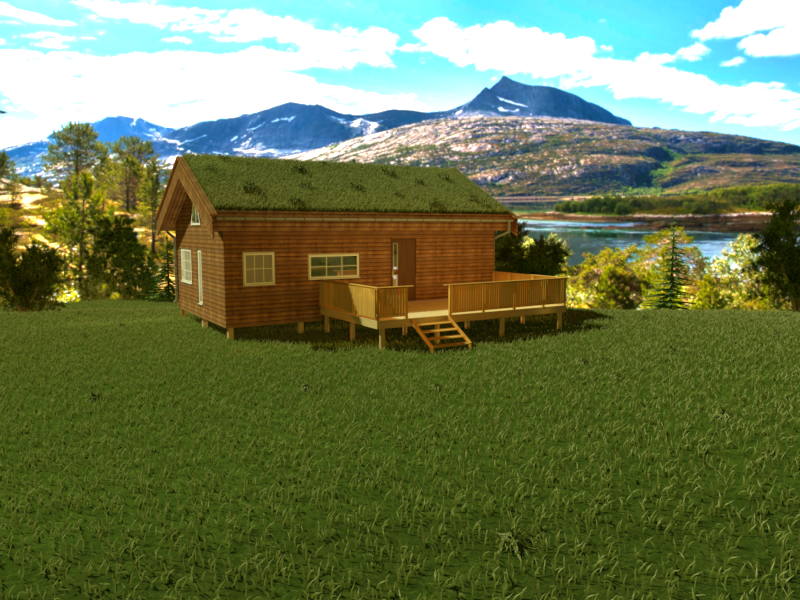
\includegraphics[scale=0.5]{Utside}\\Bygger Byggesen}
\title{Hytte ved Øyingen}
\date{17.04.2020}

\usepackage{geometry}



\begin{document}



\begin{titlingpage}
\maketitle
\end{titlingpage}

\thispagestyle{empty}
\pagebreak
\tableofcontents
\thispagestyle{empty}
\pagebreak
\clearpage
\pagenumbering{arabic}

 
\section{Beskrivelse}
\subsection{Innledning}
Tomtenummeret er 483/1/127 og er plassert på nordvestbredden av vannet Øyingen i Steinkjer kommune omtrent 258 moh. Hytta passer godt til både vinter og sommerbruk, selv om vintrene her kan bli ganske kalde. Bestemmelsene i plan- og bygningsloven og byggeforskrifter for Steinkjer kommune er oppfylt. Se dispensasjonssøknad.


\subsection{Adkomst}
Hytta ligger omtrent 550m unna nærmeste bilvei, som blir en utfordring under byggefasen. Bygging av vei vil gjøre byggingen av hytta betydelig lettere, og noe av utgiften kan deles med andre hytteboere ettersom de også vil dra nytte av en slik grusvei. I enden av adkomstveien ligger det en større parkeringsplass. Dette gjør at det ikke er behov for mer enn én parkeringsplass ved hytta.[331.130]


\subsection{Uteområde}
Uteområdet ligger idyllisk til like ved vannkanten av Øyingen. Den raske tilgangen til både vannet og naturskjønne skogsområder gjør tomta veldig attraktiv. Området har stabilt norsk klima, som vil gi kalde vintre og varme somre. I 2018 varierte temperaturen i Steinkjer mellom -20,6 $^\circ$celsius og 32,9 $^\circ$celsius. Juli er varmeste måned, med en gjennomsnittstemperatur på 18 $^\circ$celsius.[1] Utenfor inngangsdøra bygges det en terrasse. Denne kan benyttes til grilling og andre sosiale aktiviteter med venner og familie.
Det er spredt vegetasjon rundt hytta, som gjør at tomten er mer utsatt for hardt vær og vind. Dette har det blitt tatt høyde for ved utregning av blant annet vindlast.[471.043]

\pagebreak
\section{Generelt}
Snølasten i området ble beregnet til å være 4,5 $kN/m$. Denne verdien ble brukt for å regne ut Sd, som igjen ble brukt videre for å finne nødvendige dimensjoner for takbjelkene.[471.023]

Hytta er bygd etter TEK17 sine energikrav og klassifiseres i risikoklasse 4 og brannklasse 1.[473.101]

Hytta har 2 soverom i første etasje, med ekstra sengeplass på hemsen. Til sammen har hytta 6 sengeplasser, 2 på hvert rom. Hytta har ikke noe teknisk rom, men på baksiden settes det opp en bod som kan brukes til oppbevaring av en liten varmtvannstank og diverse utstyr.[331.130]

Terrassen er plassert på østsiden av huset slik at man kan nyte kaffen sin i morgensolen om somrene. Vinduet i enden av gangen hjelper til å gi hytta ekstra lys i løpet av dagen. Store vinduer i fellesareal bidrar til å gi hytta lys og varme. Med tanke på solens bevegelse over himmelen burde egentlig stue og kjøkken være plassert i andre enden av hytta for å få full utnyttelse av solstrålene. Noe å ta med videre til neste prosjekt.




\subsection{Fundament og grunn}
Fundamentet til hytta skal bygges på søyler som plasseres i søylesko, som bores ned i grunnen. Dette betyr at bjelkelaget som blir med å danne fundamentet til hytta
må isoleres tilstrekkelig og treverket trykkimpregneres for å tåle værforholdene
best mulig.
Fundamentet består av 100mm trykkimpregnert massivtre, vindsperre, 198mm isolert (mineralull) bjelkelag, oppfôring med 98mm mineralull og 36mm heltre tilfarere.[521.011][2]
Dekkes med dampsperre og parkett, mens bad og WC dekkes med mørke fliser i stedet for parkett. På kjøkkenet og i inngangspartiet legges det mørk skiferstein.
Samlet U-verdi på omtrent 0.12 $W/m^2K$.
Grunnforholdene i nærheten består av mye berggrunn, som gjør at det eventuelt må sprenges for å plassere huset direkte på grunn. Det ble derfor bestemt at huset plasseres på søyler. Avstanden mellom grunnen og fundamentet blir omtrent 370mm. Se dispensasjonssøknad.

\subsection{Bjelkelag}
Bygget har tre forskjellige bjelkelag. Alle bjelkelag legges med c/c 600mm, med avvik i endene. Det samme med kubbingen.

Fundamentet bygges i konstruksjonsvirke C24 med dimensjonene 48x198mm over et 100mm tykt lag av massivtre.

I bjelkelaget til hemsen brukes konstruksjonsvirke med fasthetsklasse C18 og har dimensjonene 48x198mm. Det er legges bærebjelke midt i bjelkelaget som støttes opp av den bærende innerveggen.

Terrassen består av bjelker i konstruksjonevirke C18 med dimensjonene 48x198mm og støttes opp av søyler som festes til berggrunnen ved hjelp av søylesko. Søylene støtter også opp under bærebjelken langs midten av bjelkelaget.[520.222][2]


\subsection{Yttervegger, dragere og søyler}
Ytterveggene består av en ytre kledning av liggende trebord i en mørkebrun farge slik at bygget skal passe det tradisjonelle hytteutseendet. 
Vindsperre plasseres under lufting
etterfulgt av et isolert stenderverk på 250mm. Deretter en nedfôring på 50mm etterfulgt av dampsperre og innvendig liggende trebord. U-verdien til
veggen er omtrent 0.17 $W/m^2K$.[471.421]


Det er plassert en drager oppunder takmøna på hytta. Fra denne drageren og ned til bjelkelaget til hemsen er det satt en søyle for å avlaste drageren.

Bindingsverket i alle vegger er plasseres i c/c 600mm.[2]

\subsection{Innervegger}
Alle innervegger, bortsett fra veggen som deler soverom 1 og bad med gangen, er satt opp med platekledning på hver side (12mm) av et isolert stenderverk (73mm).

Innerveggen som skiller sov 1 og bad med gangen er satt opp med stenderverk på 97mm i stedet for 73mm, for å støtte opp om bjelkelaget til hemsen.[2]

\subsection{Tak}
Taket er dekket av 150mm torv oppå en  knasteplate (15mm), etterfulgt av 15mm lufting. Vindsperre (2mm) legges over det 300mm tykke bjelkelaget. Det legges 50mm nedfôring med dampsperre (2mm) og innvendig liggende bordkledning (15mm). U-verdien til taket er omtrent 0.13 $W/m^2K$. Vinkelen på taket er 27 $^\circ$.
Taket dimensjoneres etter utregninger basert på egenlast (2.62 $kN/m$) og snølast (2.89 $kN/m$). Med disse verdiene ble dimensjonene til taket satt til c/c 600mm med 73x198mm bjelker av C30 konstruksjonsvirke. Dette gir en total nedbøying på omtrent 5.93 mm, som er meget akseptabelt. Mønehøyden til hytta er 4751mm, mens gesimshøyden er 2777mm.[471.013][471.023][2] Se dispensasjonssøknad.

\subsection{Vinduer og dører}
Alle vinduer bygges med vannbrett under glasset og utvendig listverk. Vinduene er 3-lags, selv om dette ikke vises i vindusdetaljen (se vedlegg), med en U-verdi på omtrent 0.72 $W/m^2K$.
I første etasje utstyres alle vinduene med naturlig ventilasjon over glass.
Alle vinduer er topphengslet med unntak av vindu 1, 2, 6 og 8, som ikke kan åpnes. Hvert rom har minst ett vindu som er en godkjent rømningsvei, unntatt vindu på hems.[520.391]

Ytterdøren har en U-verdi på 0.82 $W/m^2K$ og har slagretning utover for lettere rømning ved brann

\subsection{Trapper og stige}

Det finnes to trapper og én stige i hytta. De to trappene er utendørs og går fra grunnen til terrassen og fra grunn til boden. Inne i hytta settes det opp en stige som festes til hemsen for å spare plass. Trappene og stigen er av tre, og trappene er i tillegg trykkimpregnerte for lengre holdbarhet.

\pagebreak
\section{Tekniske løsninger}
Ettersom at det ikke er innlagt elektrisitet eller vann så må det installeres et system for å gi hytta både strøm og vann.

\subsection{Elektrisitet}
Det vil bli satt opp en liten vindturbin på tomta som har en effekt på 600W, ettersom vindforholdene på tomta virker gunstige nok til at dette. Vindturbinen er koblet til batterier som installeres i boden og derfra supplerer hytta med strøm når det trengs.

\subsection{Vann og avløp}
Med tanke på at det er dårlig fremkommelighet for større kjøretøy så vil det være vanskelig å bore etter grunnvann. 
Det mest hensiktsmessige blir derfor å pumpe vann opp fra Øyingen og rense dette gjennom et filter som monteres på veggen av hytta. Pumpa drives av strøm fra batteriene og vindturbinen.[515.235]
I nærheten av hytta lages det en filterkum som renser gråvannet før det slippes ut i grunnen. Det installeres et Jets toalett som bruker meget lite vann. Avløpsvannet samles i en tank på omtrent 2000 liter. Denne tanken plasseres i nærheten av boden og tømmes av kommunen omtrent annenhvert år, avhengig av bruk.[553.456]

\subsection{Varme}
Varmen i hytta vil hovedsaklig komme fra brukerne og elektriske apparater. I spesielt kalde perioder kan det suppleres med elektrisk panelovn eller mobil gassovn. Bad og WC vil varmes opp av varmekabler i gulvet.


\pagebreak
\section{Arealer}

	\begin{tabbing}

Bebygd areal (BYA): \hspace{20em}\=88,56 $m^2$ \\
Bruttoareal (BTA): \>94,32 $m^2$\\
Nettoareal (NTA): \> 55,7 $m^2$\\
Bruksareal (BRA):\> 77,97 $m^2$\\
Primærrom(p-rom):\> 55,22 $m^2$\\
Tomteareal:\>168 $m^2$\\
BRA\%: \> 0,46 \% \\
BYA\%: \>0,53 \% \\
	\end{tabbing}

I utregningen av BTA og BRA ble hele gulvet på hemsen tatt med i beregningene, mens i utregningen av NTA og p-rom ble kun området vist på møbleringsplanen for hemsen brukt.



\pagebreak
\section{Kalkyle}

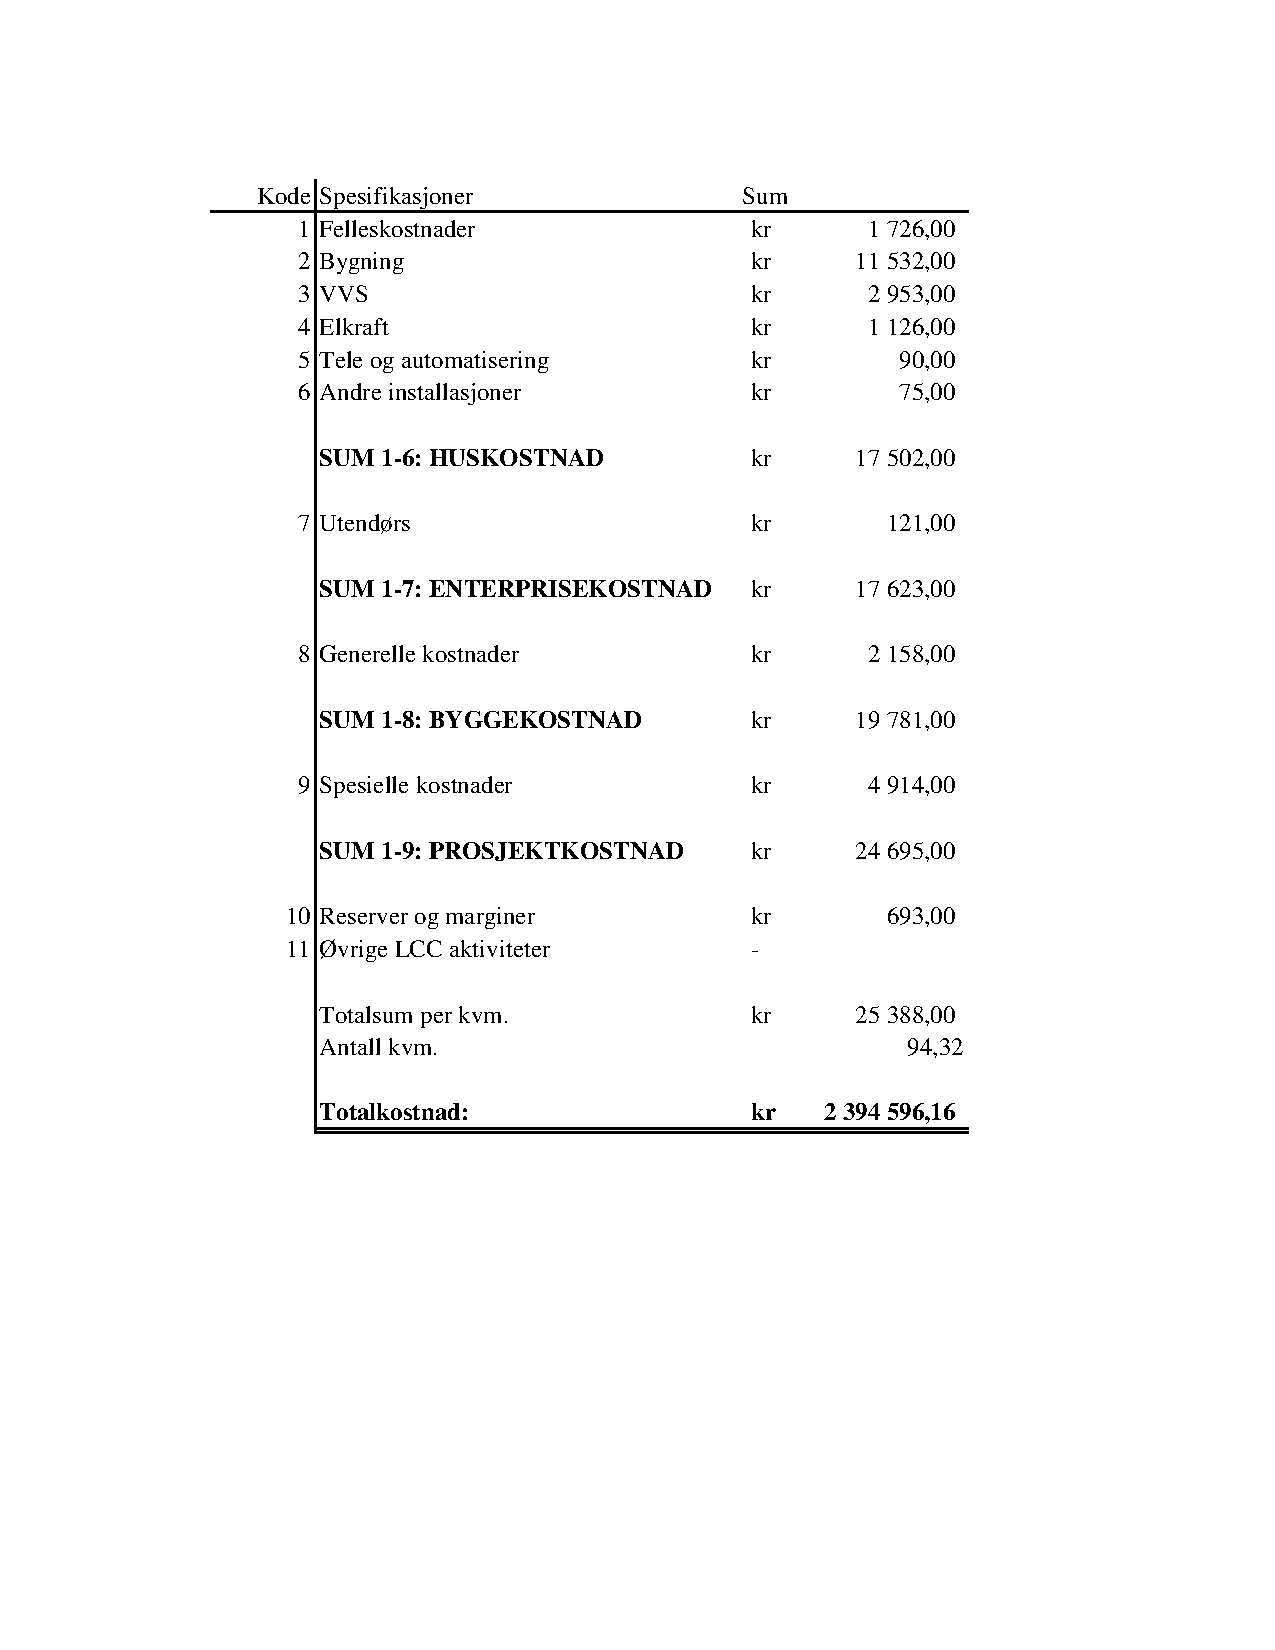
\includepdf[pages=-]{Kalkyle}

\pagebreak
\section{Kilder}
\href{http://www.byggforsk.no}{\textbf{Byggforskserien}}
\begin{itemize}
	\item 471.023 Snølast på tak. Dimensjonerende laster
	\item 471.043 Vindlaster på bygninger
	\item 331.130 Frittliggende hytter
	\item 515.235 Enkle vannforsyningsanlegg for fritidsboliger
	\item 553.456 Alternative klosettanlegg
	\item 521.011 Valg av fundamentering og konstruksjoner mot grunnen
	\item 471.421 U-verdier. Vegger over terreng-massivtre
	\item 471.013 U-verdier. Tak
	\item520.391 Rømning via vindu. Krav og utforming
	\item 473.101 Energikrav til bygninger. Oversikt
	\item 520.222 Bjelker av tre. Dimensjonering

\end{itemize}

\textbf{Øvrige kilder:}
\begin{itemize}
	\item[1]\href{https://www.yr.no/nb/historikk/graf/1-2296935/Norge/Tr\%C3\%B8ndelag/Steinkjer/Steinkjer?q=2018}{Yr.no historisk temperatur Steinkjer}
	\item[2] Håndbok 5 Trehus 
\end{itemize}


\pagebreak
\section{Vedlegg}


\subsection{Dispensasjonssøknad}
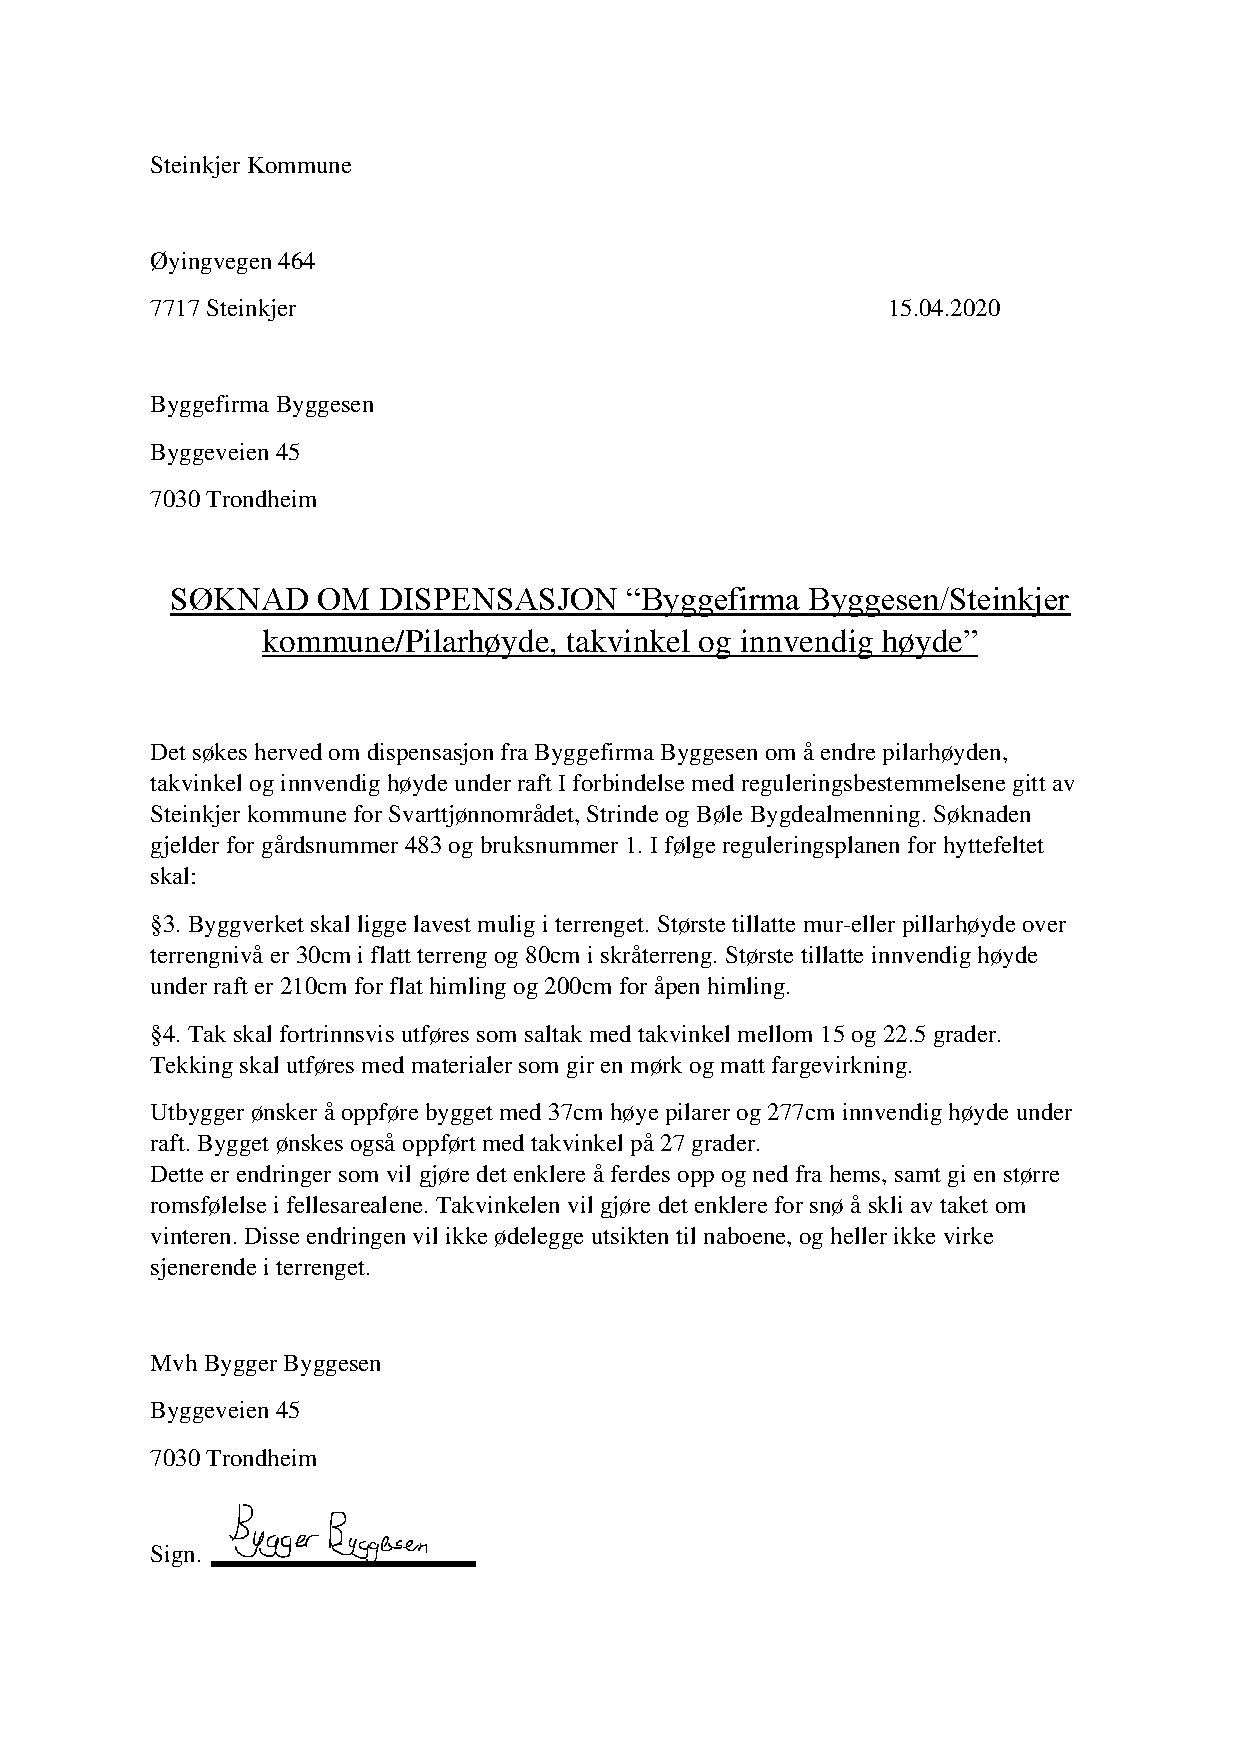
\includepdf[pages=-]{Soknad}

\pagebreak
\subsection{Skjema: 5174}
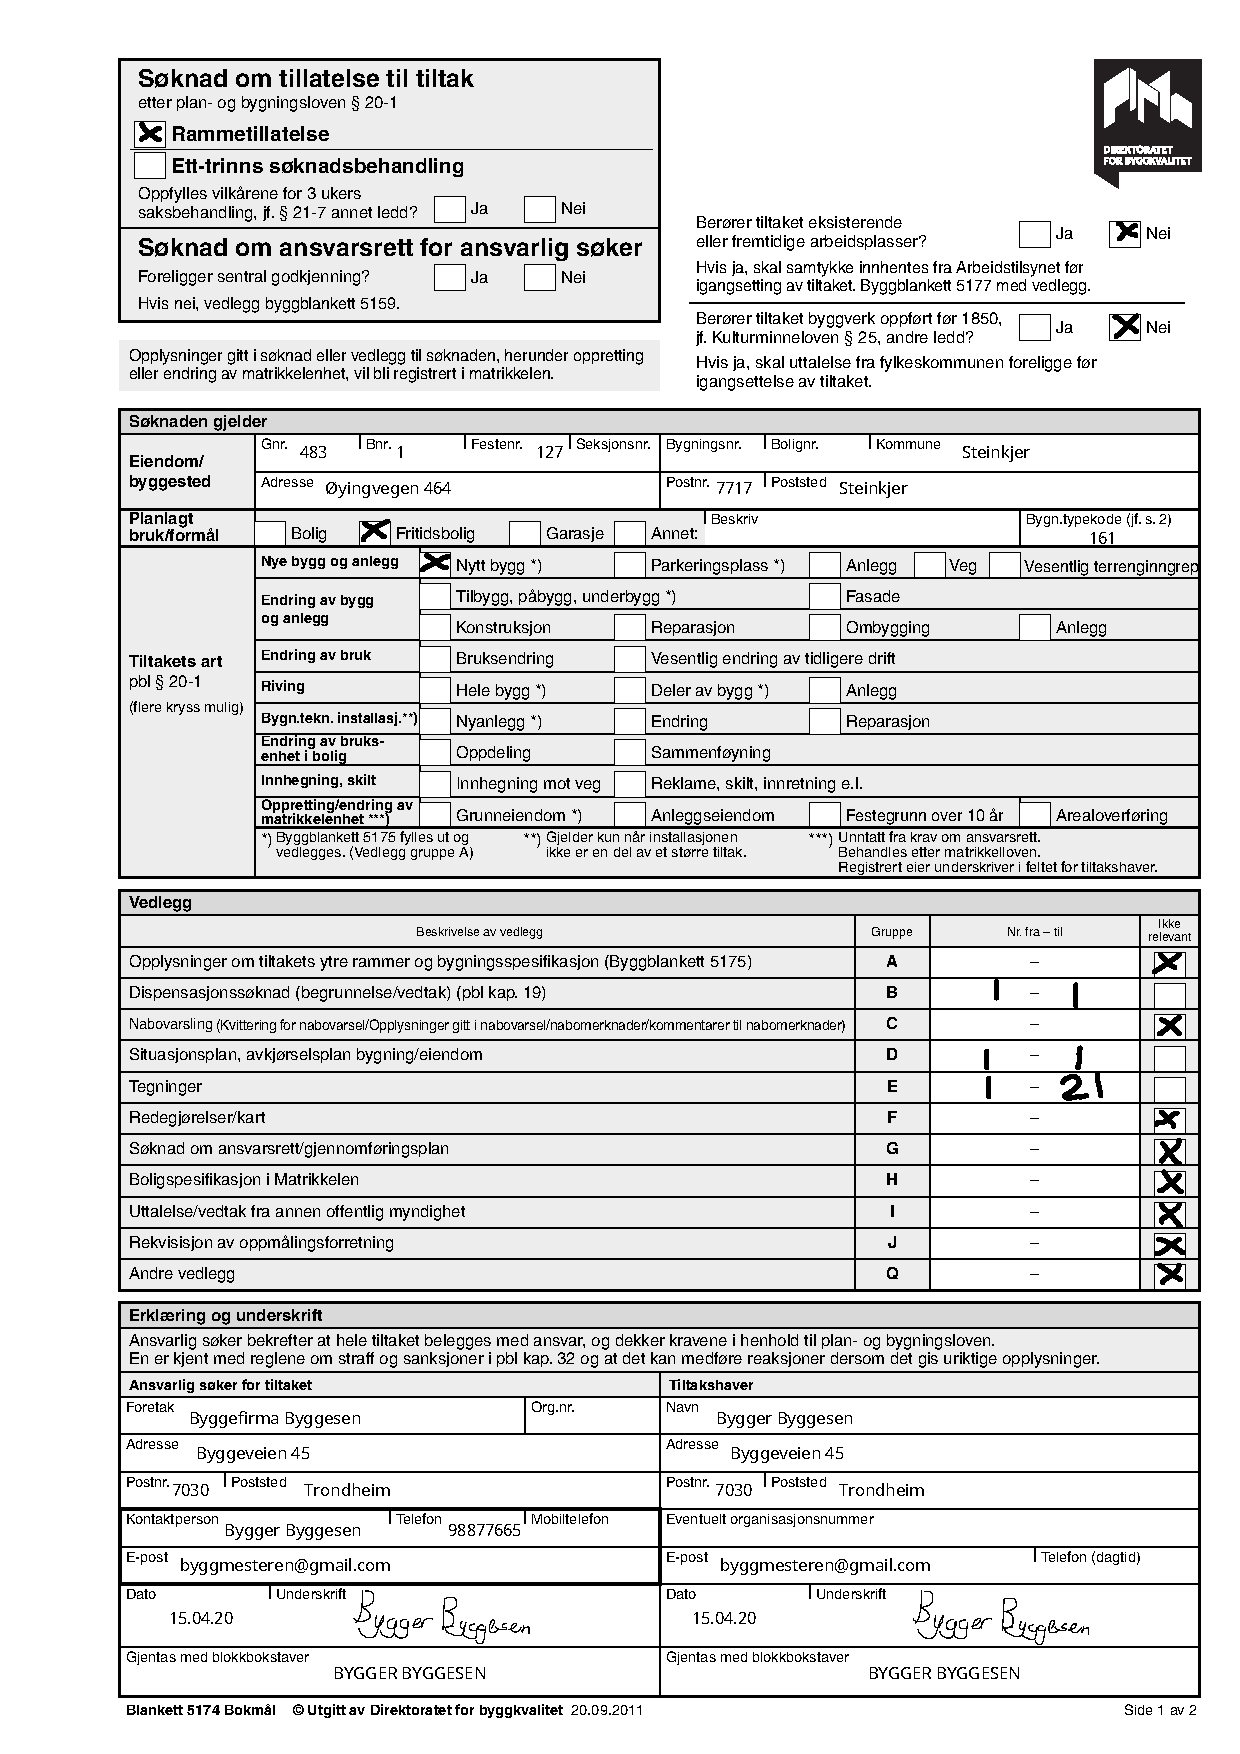
\includepdf{5174}

\pagebreak
\subsection{Vindusskjema}
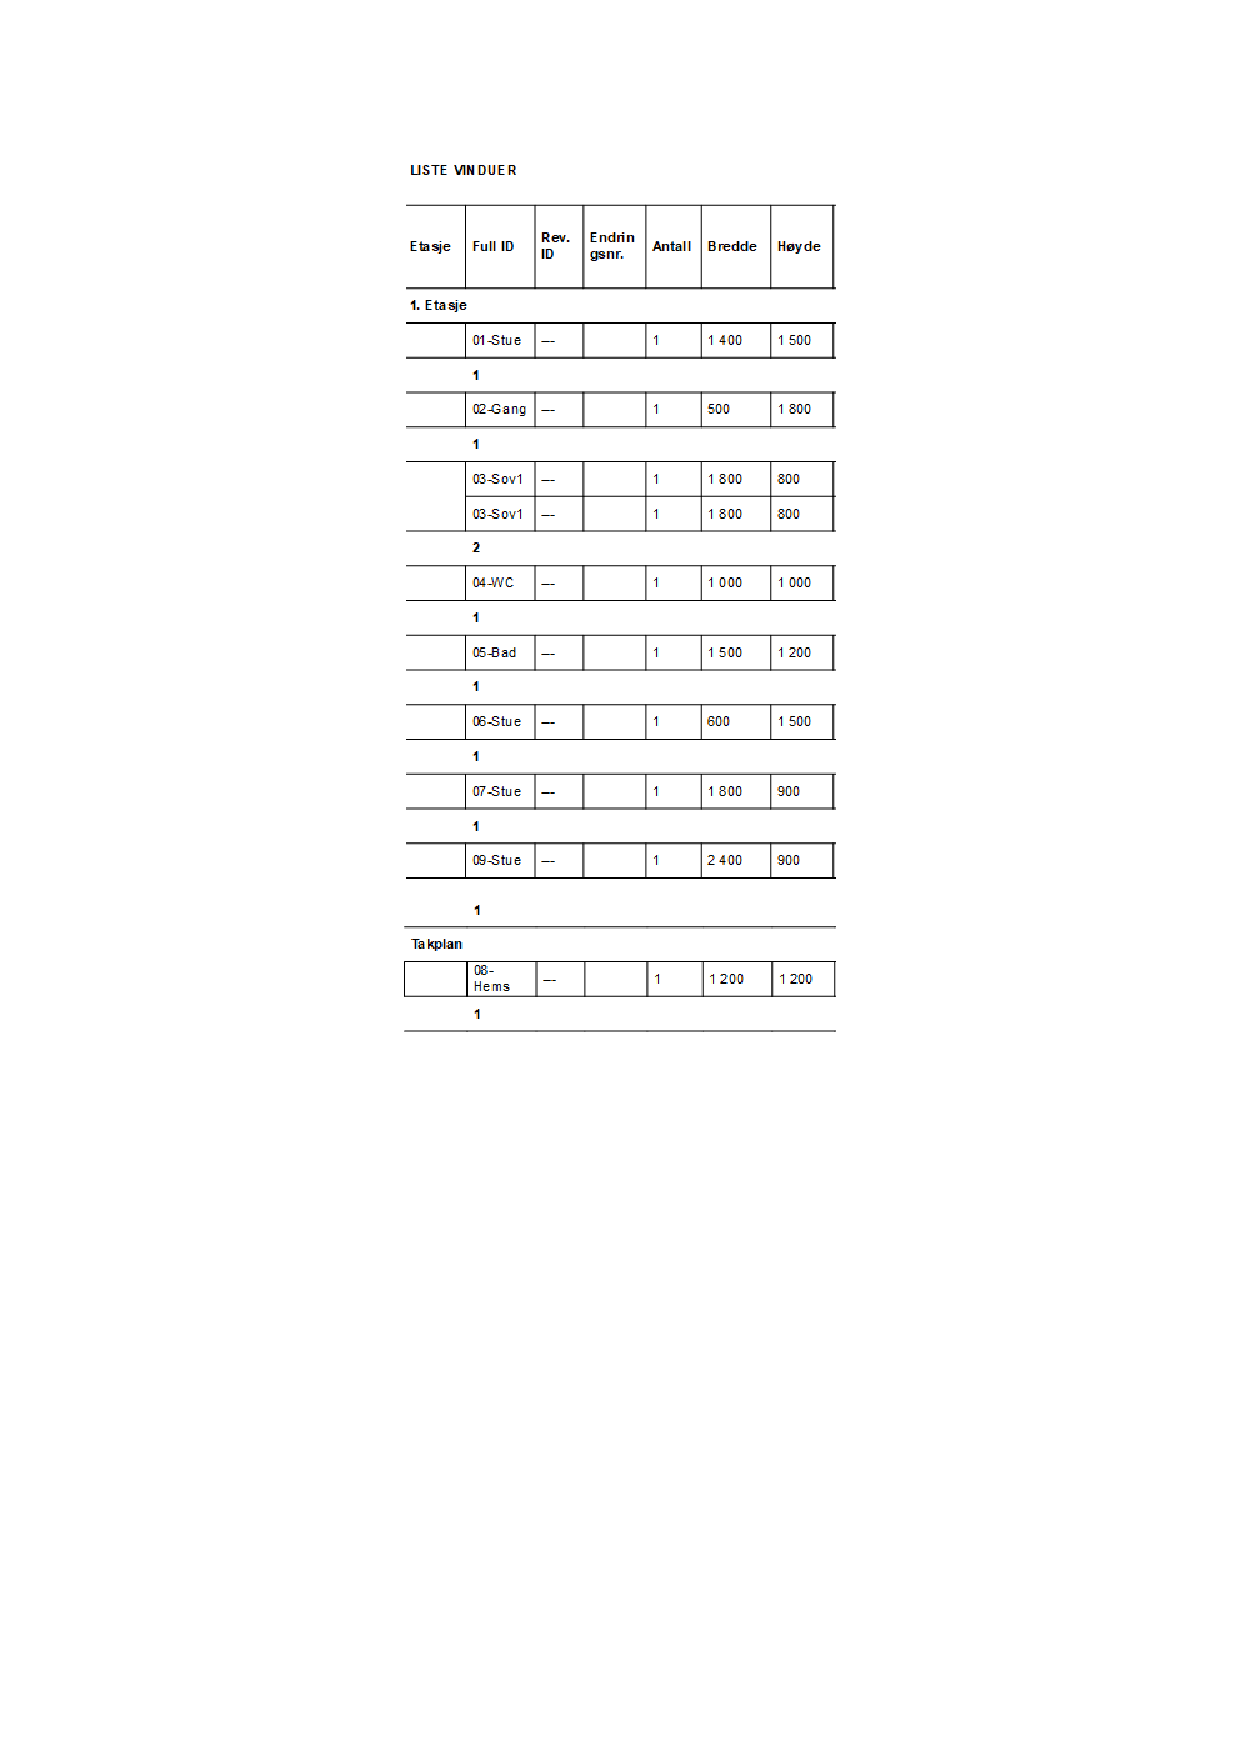
\includepdf[pages=-]{Vindusliste}


\pagebreak
\subsection{Tegningsliste}
Tegning 2.1 plantegning 1.etasje viser målestokk 1:5, men er i realiteten målestokk 1:50.
På tegning 4.1 Fasade sørvest synes ikke taket til boden. På samme tegning synes heller ikke bordene som egentlig er lagt oppå takskjegget på kortendene.
Tegning 4.2 Fasade nordøst viser ikke bjelkelaget til terrassen. Dette vises heller ikke på tegningene 4.3 og 4.4.
Fasade nordvest og sørøst viser noen av forkantsborda i vertikal orientering. Alle borda skal egentlig være horisontalorientert.


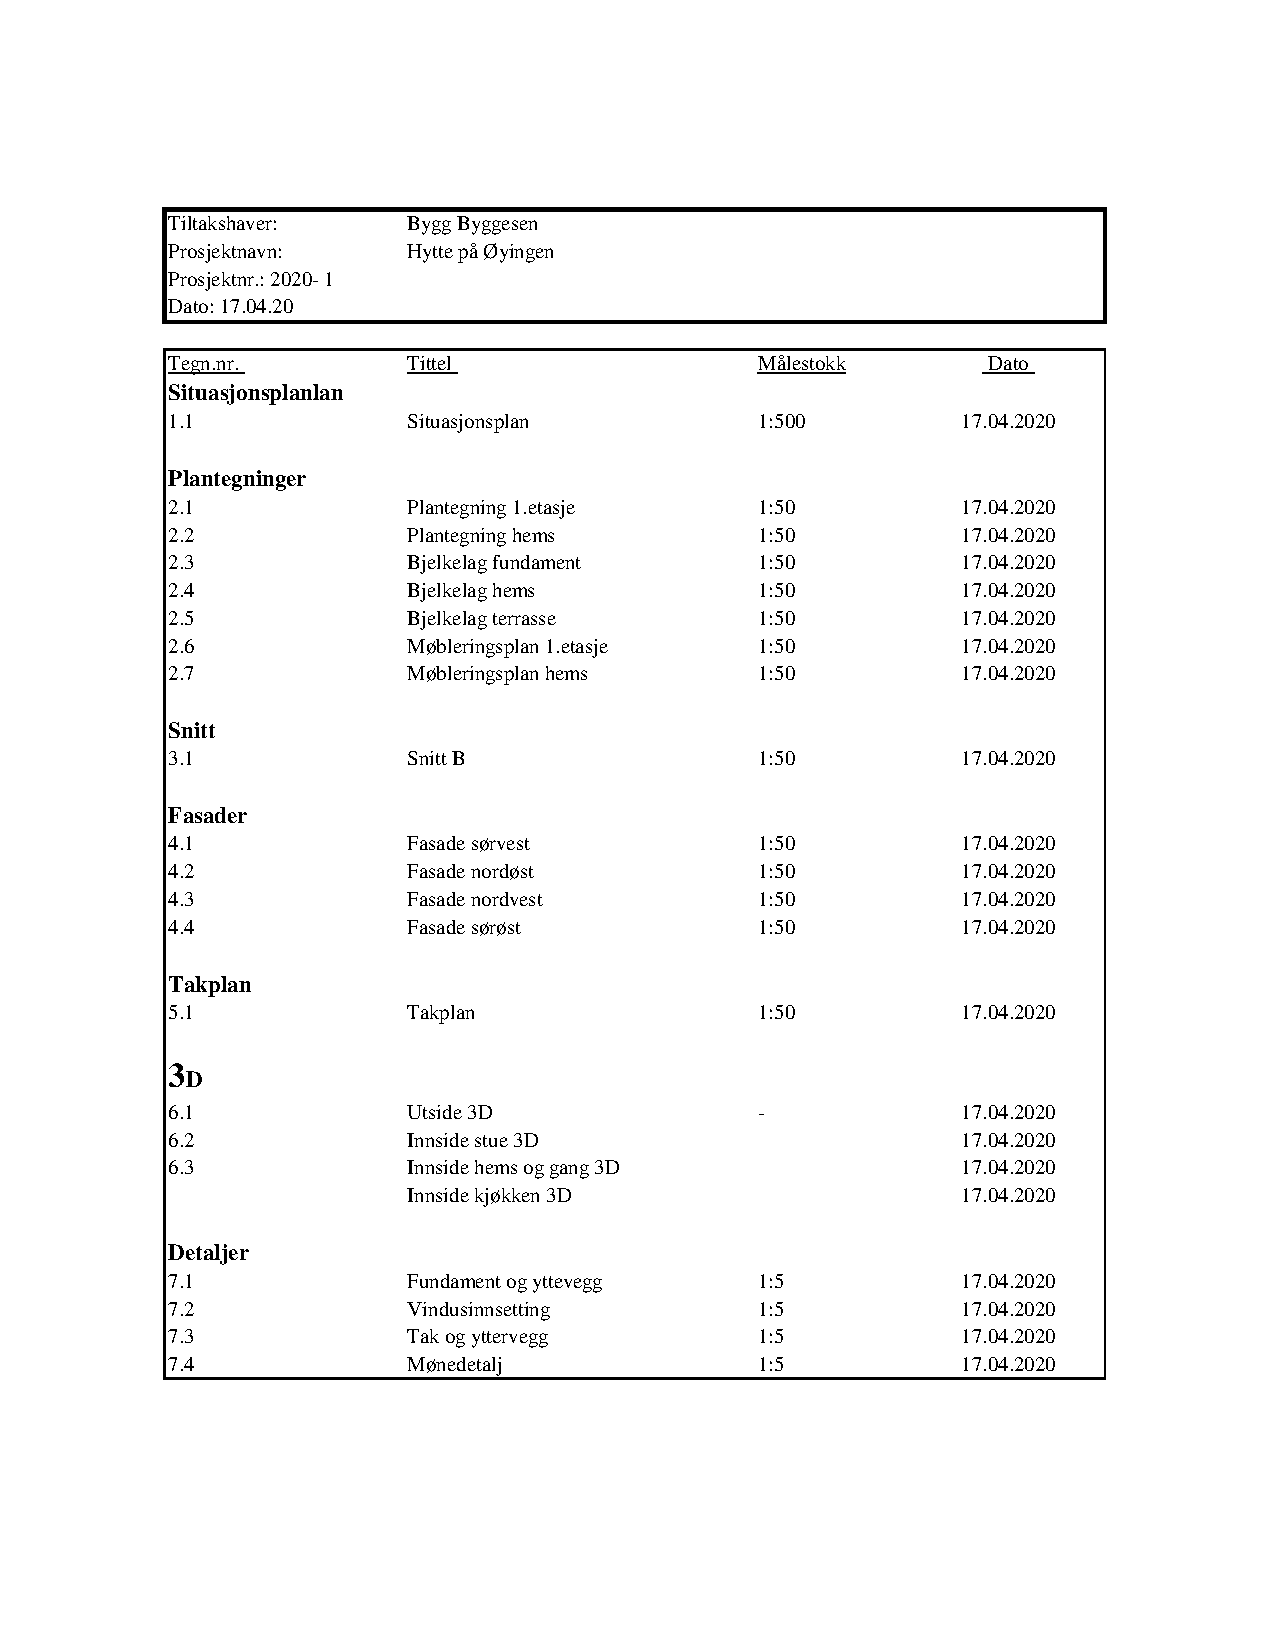
\includepdf[pages=-]{Tegningsliste}






	
	
	
	
	
	
	
	
\end{document}